\chapter{Diseño e Implementación}
\label{cap:capitulo4}

El objetivo de este \ac{TFG} es desarrollar un sistema de conducción autónoma capaz de realizar seguimiento de carril, control adaptativo al tráfico y maniobras de adelantamiento completas de manera segura en un entorno simulado y controlado. En este capítulo, se establecen primero los fundamentos de la percepción, definiendo qué elementos del entorno pueden ser detectados y qué información estará disponible para los modelos de control. A continuación, se implementa un sistema de conducción autónoma tradicional basado en el seguimiento de carril mediante un controlador \ac{PID}. Posteriormente, se exploran algunos algoritmos de \ac{DRL}) aplicados a la conducción autónoma, desarrollando y evaluando distintos modelos para la generación de comportamientos inteligentes. Finalmente, se lleva a cabo un análisis comparativo de los diferentes enfoques implementados, destacando sus ventajas e inconvenientes en el contexto de la conducción autónoma en un escenario de carreras.

\section{Arquitectura general}

El simulador CARLA nos proporciona un entorno de simulación avanzado que incluye el vehículo a controlar, la generación de tráfico, circuitos de prueba, así como sensores y actuadores simulados.

Entre los sensores disponibles contamos con cámaras y sensores \ac{LiDAR}, los cuales permiten obtener información detallada del entorno. Estos datos son procesados en el bloque de percepción, donde se aplican herramientas avanzadas de detección de carril y segmentación semántica sobre las imágenes capturadas, así como un tratamiento inteligente de los datos provenientes del \ac{LiDAR}. El objetivo de este procesamiento es extraer información relevante y simplificada, que servirá como observaciones para los modelos de conducción autónoma.

Los modelos de conducción autónoma, tanto los tradicionales como los basados en \ac{DRL}, procesan esta información para aprender a tomar decisiones óptimas y robustas en tiempo real. Estas decisiones se aplican directamente a los actuadores del vehículo dentro del simulador CARLA.

El comportamiento resultante de estos procesos, así como las relaciones entre los distintos bloques funcionales del sistema, pueden observarse reflejados en el diagrama de diseño \ref{fig:arch}.

\begin{figure}[ht]
  \centering
  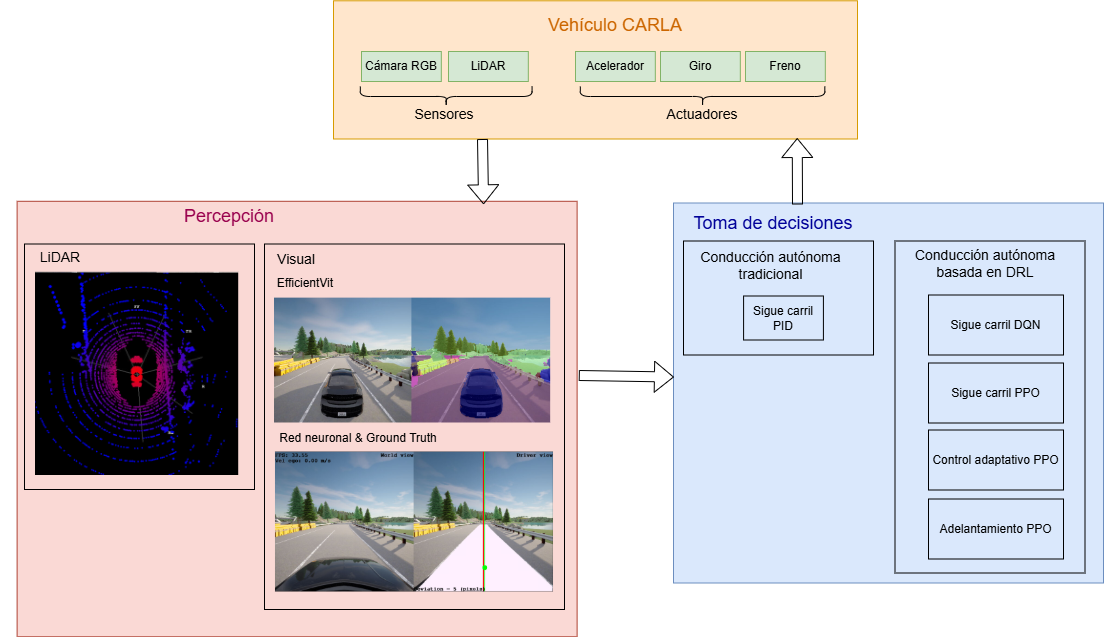
\includegraphics[width=16cm]{figs/Diseño/arquitectura.png}
  \caption{Arquitectura general.}
  \label{fig:arch}
\end{figure}

\section{Percepción visual}

La percepción visual se basa en las imágenes captadas por una cámara RGB, un sensor simulado en CARLA, con una resolución de 512 x 512 píxeles. Esta cámara se coloca con una perspectiva similar a la de un conductor. En esta sección, veremos cómo, a partir de esa información y aplicando diversas herramientas, es posible identificar el carril y segmentar la imagen.

\subsection{Detección de carril}

El objetivo es utilizar cada una de las herramientas de detección de carril para identificar los límites derecho e izquierdo del carril. Ademas, se definide una altura máxima para la detección del carril, creando así la forma de un trapecio. Al unir los puntos a la misma altura, podemos obtener el área del carril, su centro de masas y la desviación del coche con respecto al carril, considerando el centro de la imagen como el centro de nuestro vehículo.

\begin{code}[h]
\begin{lstlisting}[language=Python]

for i in range(limitis_for[0], limitis_for[1]): # Altura
	if not self._lane_network: # Ground truth
		x_left, y = self._lane_left[i]
		x_right, _ = self._lane_right[i]
	else: # Deteccion de carril DL
		y = i
		x_left = max(int(y * coef_left[0] + coef_left[1]), 0)
		x_right = min(int(y * coef_right[0] + coef_right[1]) + 1, SIZE_CAMERA - 1)

	if x_left < x_right:
		img[y, x_left:x_right] = (255, 240, 255)
\end{lstlisting}
\caption[Detección y cálculo de la superfice del carril]{Detección y cálculo de la superfice del carrill.}
\label{code:detectar_carril}
\end{code}

Teniendo los puntos límite del carril en todas las alturas, también es sencillo calcular \textit{n} puntos de cada línea del carril igualmente espaciados en el eje y. En la Figura \ref{fig:puntos_carril}, se muestra un ejemplo de cómo se obtienen diez puntos de cada línea del carril. Estos puntos, junto con el centro de masas, el área y la desviación del carril, constituyen una representación simplificada del carril para el modelo de conducción autónoma.

\begin{figure}[ht]
  \centering
  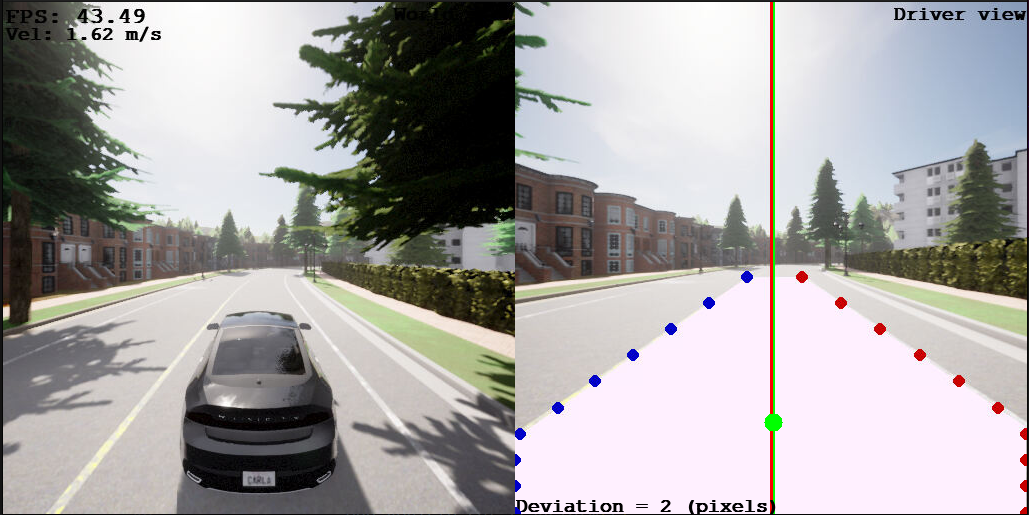
\includegraphics[width=11cm]{figs/Diseño/lane10.png}
  \caption{Representación del carril: superficie, centro de masas, desviación y puntos de sus líneas.}
  \label{fig:puntos_carril}
\end{figure}

\subsubsection{Modelo basado en \ac{DL}}

El modelo de \ac{DL} para la detección de carril procesa imágenes de 512 x 1024 píxeles. Para ello, primero creamos una imagen vacía y colocamos la del carril en el centro. Esta imagen se pasa como entrada al modelo, el cual devuelve dos máscaras que definen las líneas del carril. Para mejorar la detección, especialmente en situaciones donde las líneas están discontinuas o cuando la red neuronal devuelve líneas fragmentadas o incompletas, aplicamos regresión lineal a los puntos obtenidos para cada línea. Este procedimiento nos permite calcular los coeficientes de las rectas que mejor se ajustan a esos puntos, y con ello, conocer sus límites.

\begin{figure}[ht]
  \centering
  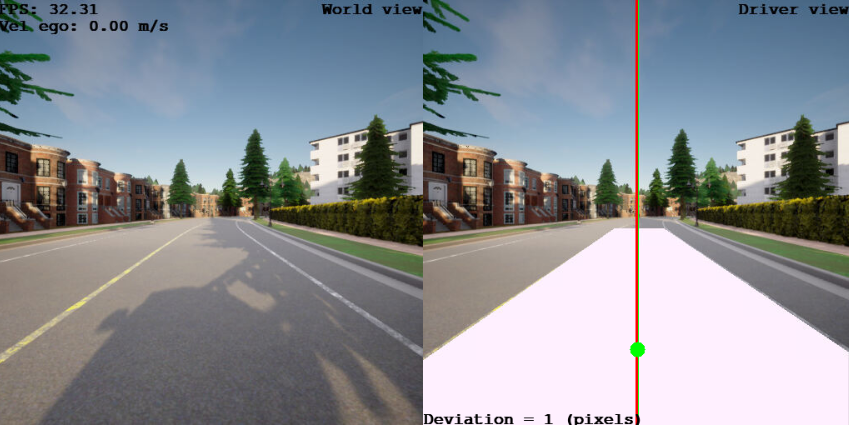
\includegraphics[width=11cm]{figs/Diseño/red_neuronal_carril.png}
  \caption{Detección de carril basada en \ac{DL}.}
  \label{fig:dl_final_carril}
\end{figure}

A pesar de esta regresión, hemos implementado una técnica para eliminar los \textit{outliers} de cada máscara. Solo conservamos los puntos que caen dentro de un umbral determinado a partir de la medida anterior. En la Figura \ref{fig:outliers}, se ilustra este proceso utilizando la siguiente codificación de colores:

\begin{figure}[ht]
  \centering
  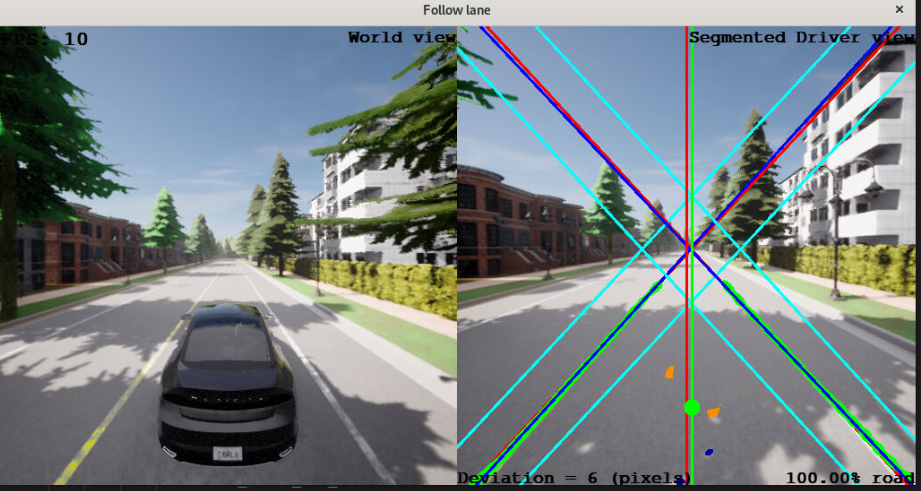
\includegraphics[width=11cm]{figs/Diseño/remove_outliers.png}
  \caption{Eliminación de \textit{outliers} en la detección de carril basada en \ac{DL}.}
  \label{fig:outliers}
\end{figure}

\begin{itemize}
		\item Las líneas rojas en forma de cruz representan las dos detecciones de cada línea de carril previas.
		\item Las líneas cian que rodean a las anteriores delimitan la zona válida.
		\item Los puntos verdes son los puntos válidos que se tendrán en cuenta para la detección del carril, mientras que los puntos azules o naranjas representan los \textit{outliers}.
		\item Las líneas azules son el resultado de aplicar regresión lineal sobre los puntos válidos (verdes).
\end{itemize}

De esta manera, conseguimos una detección más precisa del carril. Además, se ha implementado un sistema de memoria para filtrar mediciones erróneas. Este sistema almacena las cinco últimas detecciones de las líneas, junto con el ángulo que cada una forma con la horizontal. Si el ángulo de la detección actual difiere lo suficiente de la media de los ángulos almacenados o si no se detecta ninguna línea, descartamos la medida y utilizamos la última detección válida. Si esto ocurre durante más de cinco iteraciones consecutivas, determinamos que se ha perdido el carril.

\begin{code}[h]
\begin{lstlisting}[language=Python]
index_mask = np.where(mask > self._threshold_lane_mask)
coefficients = np.polyfit(index_mask[0], index_mask[1], 1)

# Comprobar la medida
mean = np.mean(self._coefficients[:, index, 2])  
angle = math.degrees(math.atan(coefficients[0])) % 180  

if  abs(mean - angle) > MAX_ANGLE:
    self._count_mem_lane[index] += 1 
    return False  # Tomamos medida anterior
else:
    self._count_mem_lane[index] = 0  # Reiniciar contador memoria
    self._coefficients[-1, index, 0:2] = coefficients 
    self._coefficients[-1, index, 2] = angle

\end{lstlisting}
\caption[Detección de carril \ac{DL}: regresión lineal y validación de medida]{Detección de carril \ac{DL}: regresión lineal y validación de medida.}
\label{cod:dl_carril}
\end{code}

\subsubsection{Ground truth}

Una vez aplicado el \textit{ground thruth}, obtenemos algunos puntos del límites del carril, pero no todos. Para obtener los límites completos del carril, utilizamos la función \textit{pygame.draw.lines}. Sin embargo, esta función solo devuelve el rectángulo que rodea la línea dibujada, pero no los puntos de la línea en sí. Por lo tanto, dibujamos la línea sobre una superficie negra y luego analizamos esta superficie para localizar los límites del carril en términos de píxeles. Para optimizar el rendimiento computacional, restringimos la búsqueda al área dentro del rectángulo que encierra la línea. Al encontrar un punto, detenemos la búsqueda, ya que, dado que la línea es continua, podemos asumir con certeza que en cada altura habrá un punto que marcará el límite del carril. Si buscamos el límite izquierdo, comenzamos desde el inicio de la imagen (x = 0), mientras que, si buscamos el límite derecho, empezamos desde el final de la imagen. El siguiente código ilustra este proceso:
\begin{code}[h]
\begin{lstlisting}[language=Python]

rect = pygame.draw.lines(black_surface, (255, 0, 0), False, projected_boundary, 4)
pixels = []
for y in range(rect.top, rect.bottom):
    for x in range(start, end, step):
        color = black_surface.get_at((x, y))
        if color[0] == 255:
            pixels.append((x, y)) # Limites del carril
            break

\end{lstlisting}
\caption[Identificación de puntos del carril con información de \textit{ground thruth}]{Identificación de puntos del carril con información de \textit{ground thruth}.}
\label{cod:gt_carril}
\end{code}

Como se mencionó en la sección anterior, este enfoque resulta más fiable que la detección de carril mediante \ac{DL}, ya que, a pesar de los posibles obstáculos que puedan afectar la visibilidad, es capaz de seguir detectando el carril gracias a la información obtenida directamente del simulador CARLA. Por lo tanto, esta será la técnica empleada durante los entrenamientos, ya que, en ciertos escenarios, es necesario tener un vehículo delante que pueda ocultar temporalmente las líneas del carril.

\begin{figure}[ht]
  \centering
  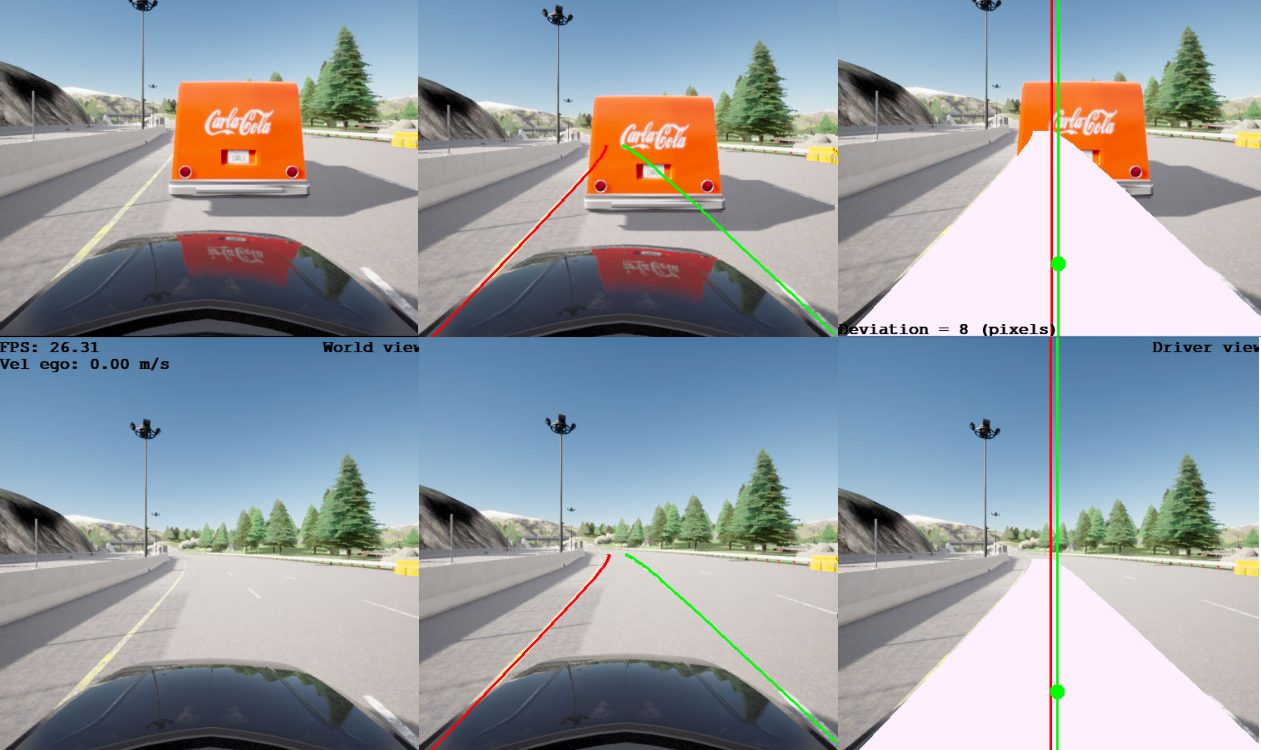
\includegraphics[width=11cm]{figs/Diseño/ground_truth.png}
  \caption{Detección de carril basada en \textit{ground thruth}.}
  \label{fig:gt_final_carril}
\end{figure}

\subsection{Segmentación la calzada}

Con la red neuronal de segmentación semántica, podemos conocer con precisión los límites y área de la calzada. Al igual que para el carril, necesitamos una representación simplificada de la misma, para ello, analizamos la máscara de segmentación que nos proporciona EfficientVit para calcular su área, centro de masas y dieciséis puntos igualmente espaciados de cada límite lateral de la calzada. Con el fin proporcionar información más valiosa al modelo, seleccionamos solo un cuarto de los puntos de la parte totalmente vertical, como se puede apreciar en la Figura \ref{fig:seg_params}. Para implementar esta funcionalidad nos hemos apoyado principalmente en la librería NumPy.

\begin{figure}[ht]
  \centering
  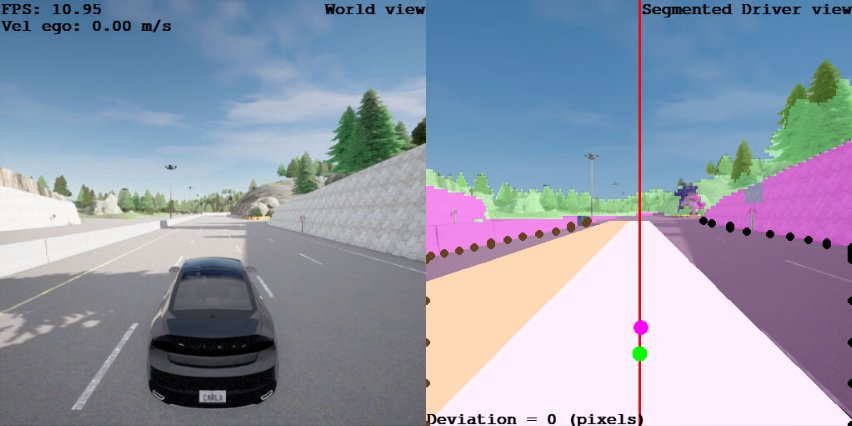
\includegraphics[width=12cm]{figs/Diseño/seg_points.png}
  \caption{Representación de la calzada: superficie, centro de masas y límites.}
  \label{fig:seg_params}
\end{figure}

También se utiliza la segmentación para saber si hay un carril a la izquierda que nos permita llevar a cabo la maniobra de adelantamiento. Para hacer esta comprobación, replicamos el carril actual a la izquierda y comprobamos que porcentaje de esta área es calzada, zona naranja en la Figura \ref{fig:seg_params}.

\section{Percepción con \ac{LiDAR}}

\section{Conducción autónoma tradiconal}
.....
\subsection{Controlador \ac{PID} para el seguimiento de carril}

\section{Conducción autónoma basada en \ac{DRL}}

Como vimos en la primera sección, el aprendizaje por refuerzo utiliza una \textit{Q-table} para encontrar las acciones que proporcionaban mayor recompensa, pero esto ya no es una forma práctica de modelar la función de transición de estado-acción, especialmente cuando el espacio de estados es muy extenso o continuo, tendríamos que explorar cada estado al menos una vez para encontrar la mejor solución. En su lugar, los algoritmos de \ac{DRL} utilizan una \textit{Q-network}, red neuronal diseñada para aprender la función que mapea estados-acciones. Esta red es capaz de estimar el valor de estados no explorados, ya que aprende las relaciones entre los diferentes pares estado-acción. En una \textit{Q-table}, los valores se almacenan en una tabla, mientras que en una \textit{Q-network} se guarda en los pesos de la red. Esta red recibe los estados del entorno como entrada y produce como salida el valor de cada acción posible. 

El \ac{DRL} es un enfoque en el que los agentes de aprendizaje por refuerzo utilizan redes neuronales para tomar decisiones. Esta combinación les permite adaptarse mejor a entornos complejos donde las reglas no son evidentes ni fácilmente definibles, como es el caso de la conducción autónoma. Dentro de los algoritmos de \ac{DRL}, existen dos tipos claramente diferenciados:

\begin{itemize}
		\item \textit{On-policy:} Son aquellos que actualizan el modelo solo con datos de la política actual, una vez que la política cambia, los datos anteriores se vuelven inservibles y se descartan.
		\item \textit{Off-policy:} Son aquellos que pueden usar cualquier dato recolectado durante el entrenamiento, independientemente de la política con la que hayan sido obtenidos.

\end{itemize}

En este \ac{TFG}, solo se han utilizado los algoritmos de \ac{DQN} y \ac{PPO}, que son \textit{off-policy} y \textit{on-policy} respectivamente \cite{drl}.

\subsection{Seguimiento de carril con DQN}

\ac{DQN} es un algoritmo de \ac{DRL} que soportar un espacio de estados complejo y continuo, pero el espacio de acciones es discreto. Las acciones en un espacio discreto son predefinidas y limitadas, es decir, no existe una continuidad entre ellas, sino que están representadas por un número finito de opciones que el agente puede elegir en cada estado.

\ac{DQN} es un algoritmo \textit{off-policy} ya que incluye una \textit{replay memory}. Esta técnica consiste en crear una memoria de reproducción de experiencias que almacena las k experiencias más recientes que un agente ha recopilado, ya que son las más relevantes, para así poder reutilizarlas. Si la memoria está llena, se descarta la experiencia más antigua para dar espacio a la más reciente. En cada paso de entrenamiento, se muestrea uno o más lotes de datos de forma aleatoria de la memoria para actualizar los parámetros de la red. El tamaño de la memoria debe ser lo suficientemente grande como para contener experiencias de diferentes episodios y políticas, lo que ayuda estabilizar y mejorar el entrenamiento. Al actualizar en cada paso del entrenamiento la red neuronal, la minimización del error entre las predicciones de la red y los valores reales se vuelve complicada. Para abordar este problema, se introduce una nueva red neural, \textit{target networ}, diseñada para aportar estabilidad al proceso de entrenamiento. La nueva red es una réplica de la red principal, \textit{policy network}, pero en lugar de actualizarla en cada paso, la igualamos a la red original cada cierto número de pasos, manteniendo un objetivo de entrenamiento constante.

Ahora que ya sabemos en qué consiste el algoritmo de \ac{DQN}, llega la hora de construir el entorno de entrenamiento para que un coche autónomo sea capaz de seguir el carril. Primero, debemos elegir el circuito de entrenamiento para nuestro modelo, para ello, hemos elegido el Town04 de CARLA, ya que incluye tramos largos y sin intersecciones. Como vemos en la Figura \ref{fig:mapa}, se han definido cuatro rutas, las rutas uno, dos y tres se utilizan durante el entrenamiento, mientras que la cuatro se usa para examinar el modelo en inferencia y comprobar si es capaz de generalizar. Cada una de estas rutas de entrenamiento comienza en una dirección distinta: curva a la derecha, línea recta y curva a la izquierda, con el fin de evitar \textit{overfitting} en el modelo.

\begin{figure}[ht]
  \centering
  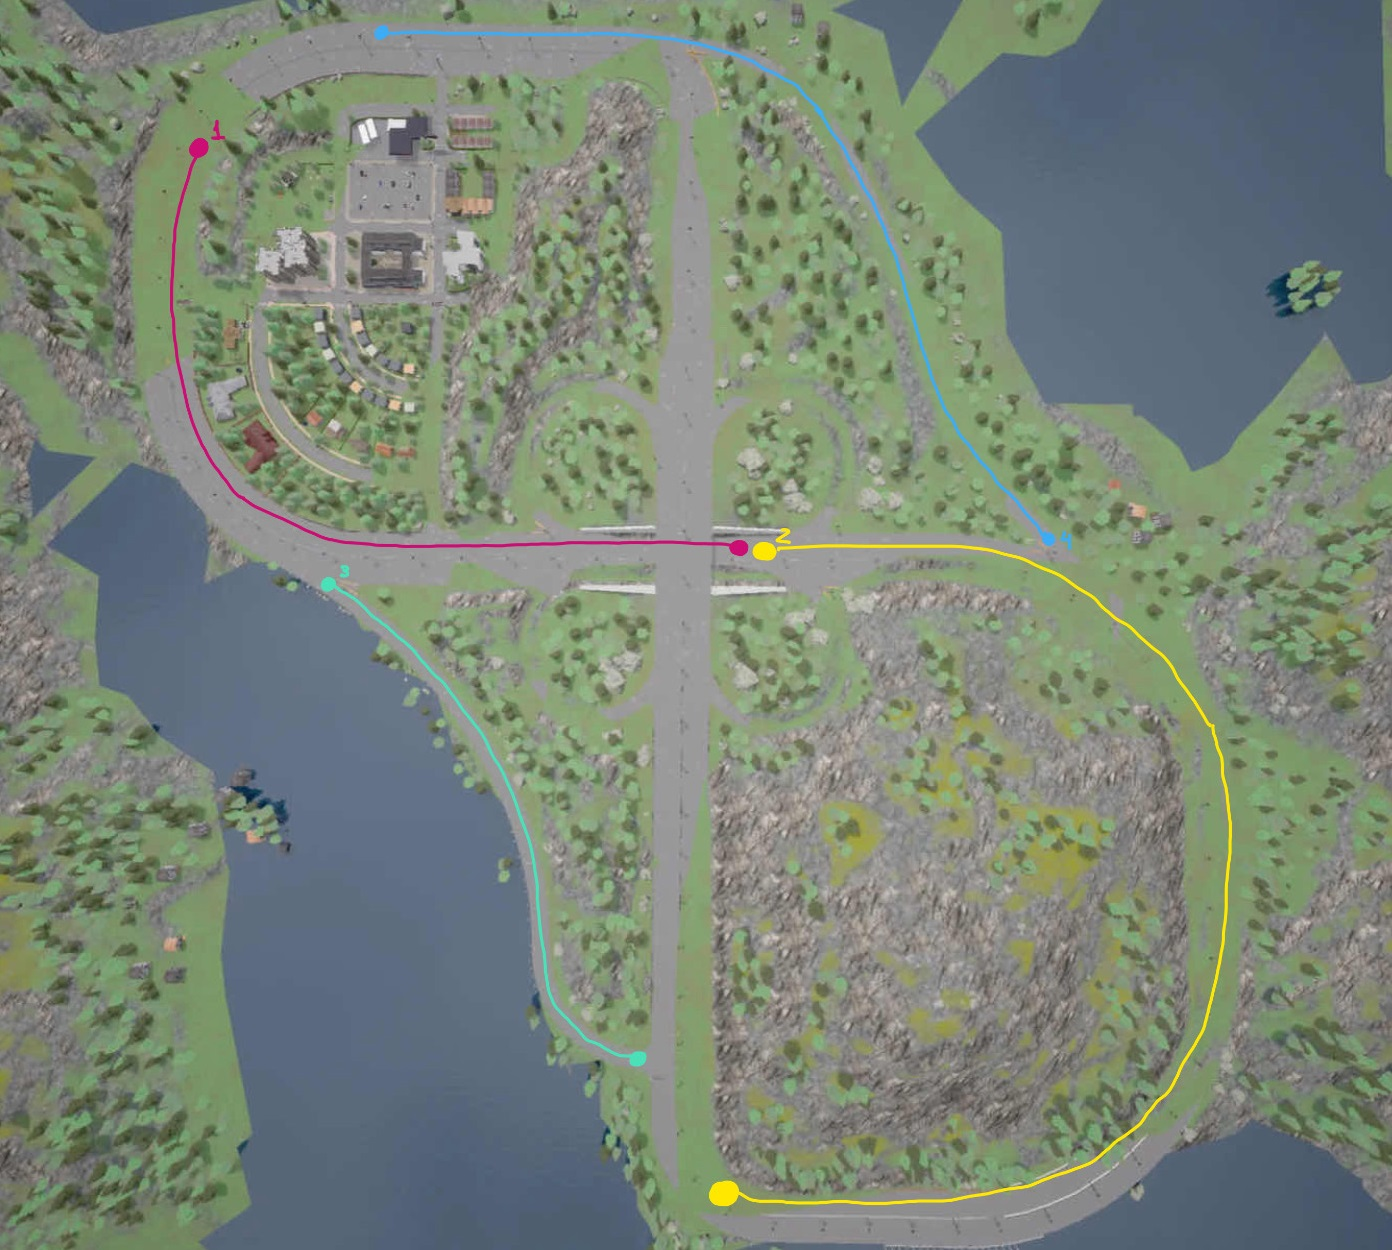
\includegraphics[width=10cm]{figs/Diseño/mapa.jpeg}
  \caption{Mapa del entorno de entrenamiento en CARLA con rutas definidas.}
  \label{fig:mapa}
\end{figure}

El vehículo autónomo incorpora los \textbf{sensores}:
\begin{itemize}
		\item Cámara RGB: se utiliza para la detección de carril. Si se pierde la percepción, sale el carril o cambia de carril se genera una excepción que se captura y finaliza el episodio.
		\item Sensor de colisión: si el coche se choca contra un elemento del entorno también detenemos el episodio.
\end{itemize}

El \textbf{espacio de observaciones} coincide con el espacio de estados y está basado en un diccionario, por lo tanto, empleamos la política \textit{MultiInputPolicy}. Las observaciones se normalizan para facilitar el aprendizaje al modelo e incluyen la siguiente información: 
\begin{itemize}
		\item Desviación del carril.
		\item Área del carril.
		\item Cinco puntos de la línea izquierda del carril.
		\item Cinco puntos de la línea derecha del carril.
		\item Centro de masas.
\end{itemize}

\begin{figure}[ht]
  \centering
  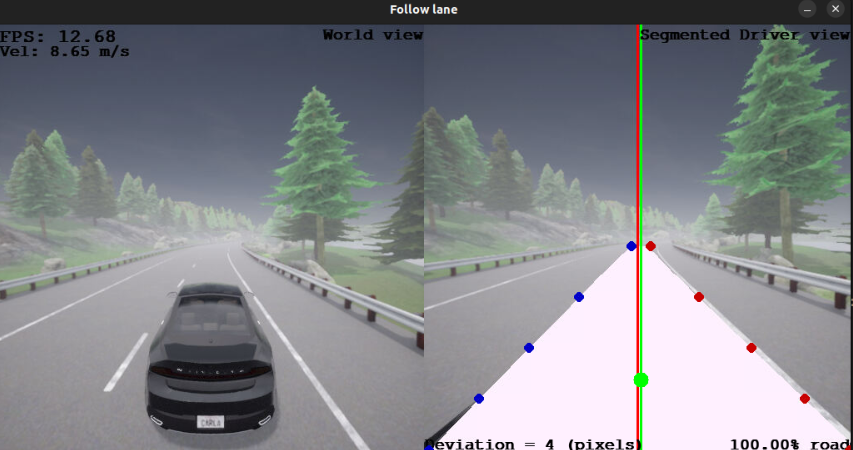
\includegraphics[width=10cm]{figs/Diseño/obs_dqn.png}
  \caption{Observaciones seguimiento de carril basado en \ac{DQN}.}
  \label{fig:dqn_obs}
\end{figure}

Como hemos mencionado al inicio, \ac{DQN} permite un \textbf{espacio de acciones discreto}. Las acciones están compuestas por un comando de acelerador y otro de giro, para combinarlo hemos seguido la regla de que, a mayor aceleración, menor es el giro. En total, se han definido 21 acciones disponibles entre las cuales el coche autónomo podrá seleccionar aquellas que maximicen la recompensa en cada situación.

\begin{code}[h]
\begin{lstlisting}[language=Python]

self.action_to_control = {
    0: (0.5, 0.0),
    1: (0.45, 0.01), 
    2: (0.45, -0.01),
    3: (0.4, 0.02),
    4: (0.4, -0.02),
    5: (0.4, 0.04),
    6: (0.4, -0.04),
    7: (0.4, 0.06),
    8: (0.4, -0.06),
    9: (0.4, 0.08),
    10: (0.4, -0.08),
    11: (0.3, 0.1),
    12: (0.3, -0.1),
    13: (0.3, 0.12),
    14: (0.3, -0.12),
    15: (0.2, 0.14),
    16: (0.2, -0.14),
    17: (0.2, 0.16),
    18: (0.2, -0.16),
    19: (0.1, 0.18),
    20: (0.1, -0.18)
}

\end{lstlisting}
\caption[Acciones disponibles para el seguimiento de carril basado en \ac{DQN}]{Acciones disponibles para el seguimiento de carril basado en \ac{DQN}.}
\label{cod:acc_dqn}
\end{code}

Nuestro objetivo es que el coche circule por el centro del carril sin desviarse, manteniendo una conducción fluida y lo más rápida posible. Para lograrlo, hemos diseñado una \textbf{función de recompensa} que se basa principalmente en la desviación del carril y en la velocidad actual del coche, normalizando y ponderando estos valores según sus respectivos pesos. Sin embargo, si el coche pierde el carril o colisiona, el episodio se detiene y se asigna una recompensa negativa.

\begin{code}[h]
\begin{lstlisting}[language=Python]
if error == None:
      # Clip deviation and velocity
      r_dev = (MAX_DEV - abs(np.clip(self._dev, -MAX_DEV, MAX_DEV))) / MAX_DEV
      r_vel = np.clip(self._velocity, 0.0, self._max_vel) / self._max_vel
      reward = 0.8 * r_dev + 0.2 * r_vel
else:
      reward = -30
\end{lstlisting}
\caption[Función de recompensa sigue-carril basado en \ac{DQN}]{Función de recompensa sigue-carril basado en \ac{DQN}.}
\label{cod:rew_dqn}
\end{code}

Para entrenar el modelo hemos utilizado un \textit{fixed\_delta\_seconds} de 50ms, lo que equivale a entrenar a 20 FPS, por lo tanto, en infrencia necesitamos operar al menos a esta velocidad. Los entrenamientos tuvieron una duración de un día y un par de horas. Tras realizar diversas pruebas experimentales, identificamos los hiperparámetros que proporcionan los mejores resultados. 
\begin{code}[h]
\begin{lstlisting}[language=Python]
learning_rate: 0.0005 # Tasa de aprendizaje
buffer_size: 20_000 # Tamano de la memoria
batch_size: 1024 # Tamano del lote
gamma: 0.85 # Factor de descuento: importancia de las recompensas futuras frente a las inmediatas
target_update_interval: 1024 # Intervalo de actualizacion de la red neuronal objetivo
train_freq: 256 # Frecuencia de entrenamiento
gradient_steps: 2 # Pasos de gradiente en cada actualizacion
exploration_fraction: 0.8 # Fraccion de exploracion
exploration_final_eps: 0.0 # Valor final de exploracion
n_timesteps: 8_000_000 # Numero total de steps

\end{lstlisting}
\caption[Hiperparámetros de entrenamiento para el sigue-carril basado en \ac{DQN}]{Hiperparámetros de entrenamiento para el sigue-carril basado en \ac{DQN}.}
\label{cod:hiper_params_dqn}
\end{code}

La frecuencia de entrenamiento resultó ser un factor clave en el proceso, al principio se utilizó un valor menor, pero los modelos no lograban converger. El ratio de exploración se reduce gradualmente durante el 80\% del entrenamiento y, a partir de ese punto, se dejan de realizar acciones aleatorias. En la siguiente gráfica, se puede observar cómo el modelo finalmente converge.
\begin{figure}[ht]
  \centering
  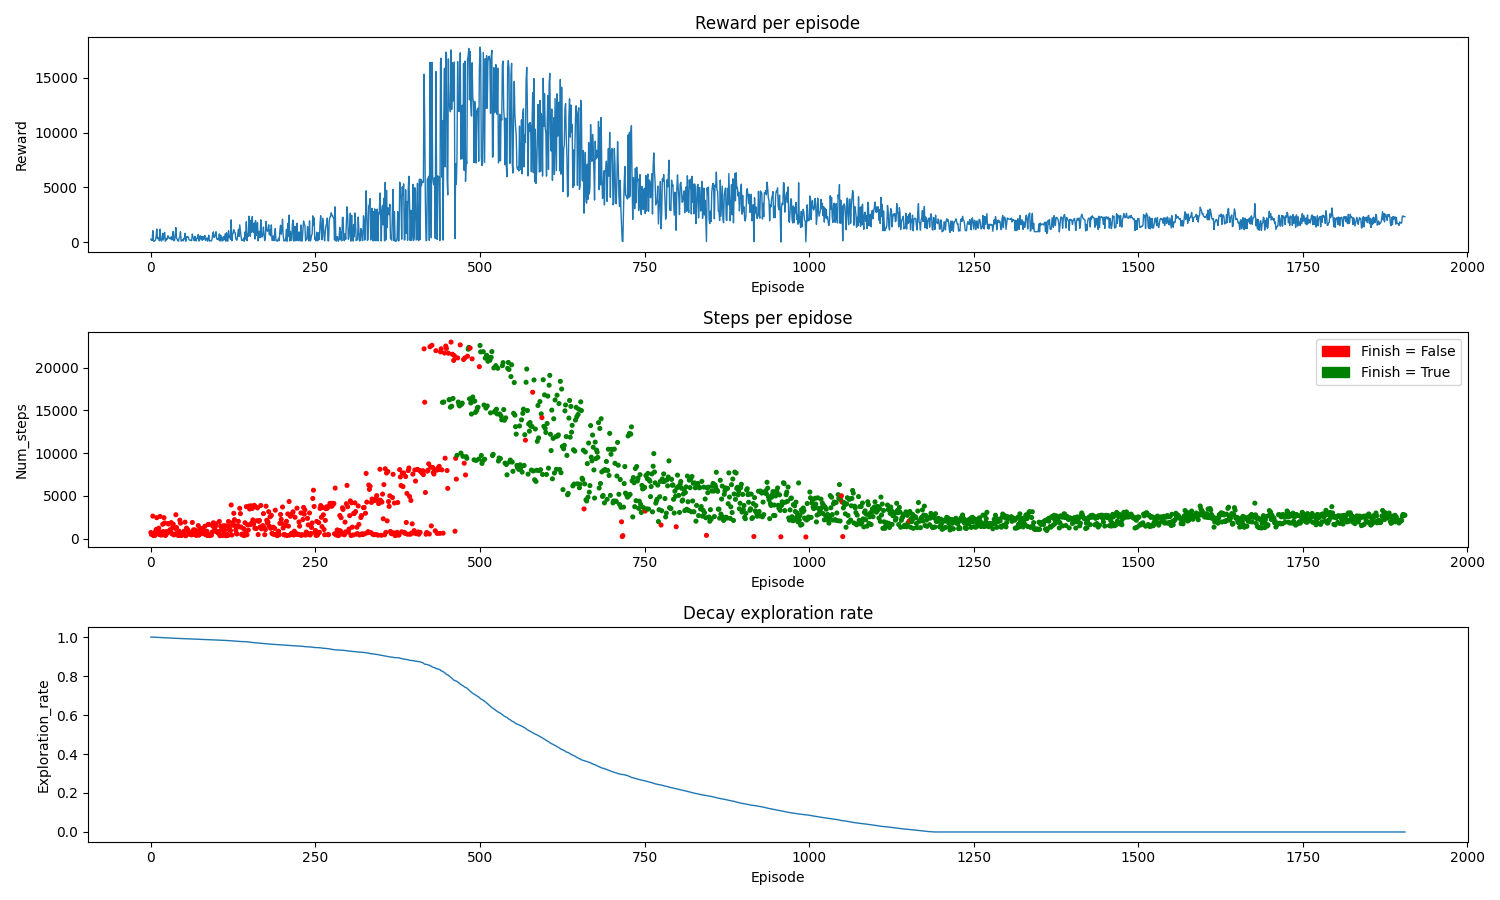
\includegraphics[width=13cm]{figs/Diseño/train_dqn.png}
  \caption{Gráfica de entrenamiento sigue-carril basado en \ac{DQN}.}
  \label{fig:train_dqn}
\end{figure}

En inferencia en un circuito visto durante los entrenamientos, se observa que el seguimiento del carril es casi perfecto. No obstante, cuando el vehículo va en línea recta, en ocasiones, se percibe un pequeño balanceo. Esto se debe a una de las limitaciones de \ac{DQN}, su espacio de acciones es discreto no permite seleccionar la acción de giro óptima en cada momento. A continuación, se presenta la información recopilada durante la inferencia. Podemos observar claramente los momentos en los que se reduce la velocidad, correspondientes a las dos curvas pronunciadas al inicio del circuito. Sin embargo, de forma general, los histogramas indican se eligen los pares de acciones más rápidos.
\begin{figure}[ht]
  \centering
  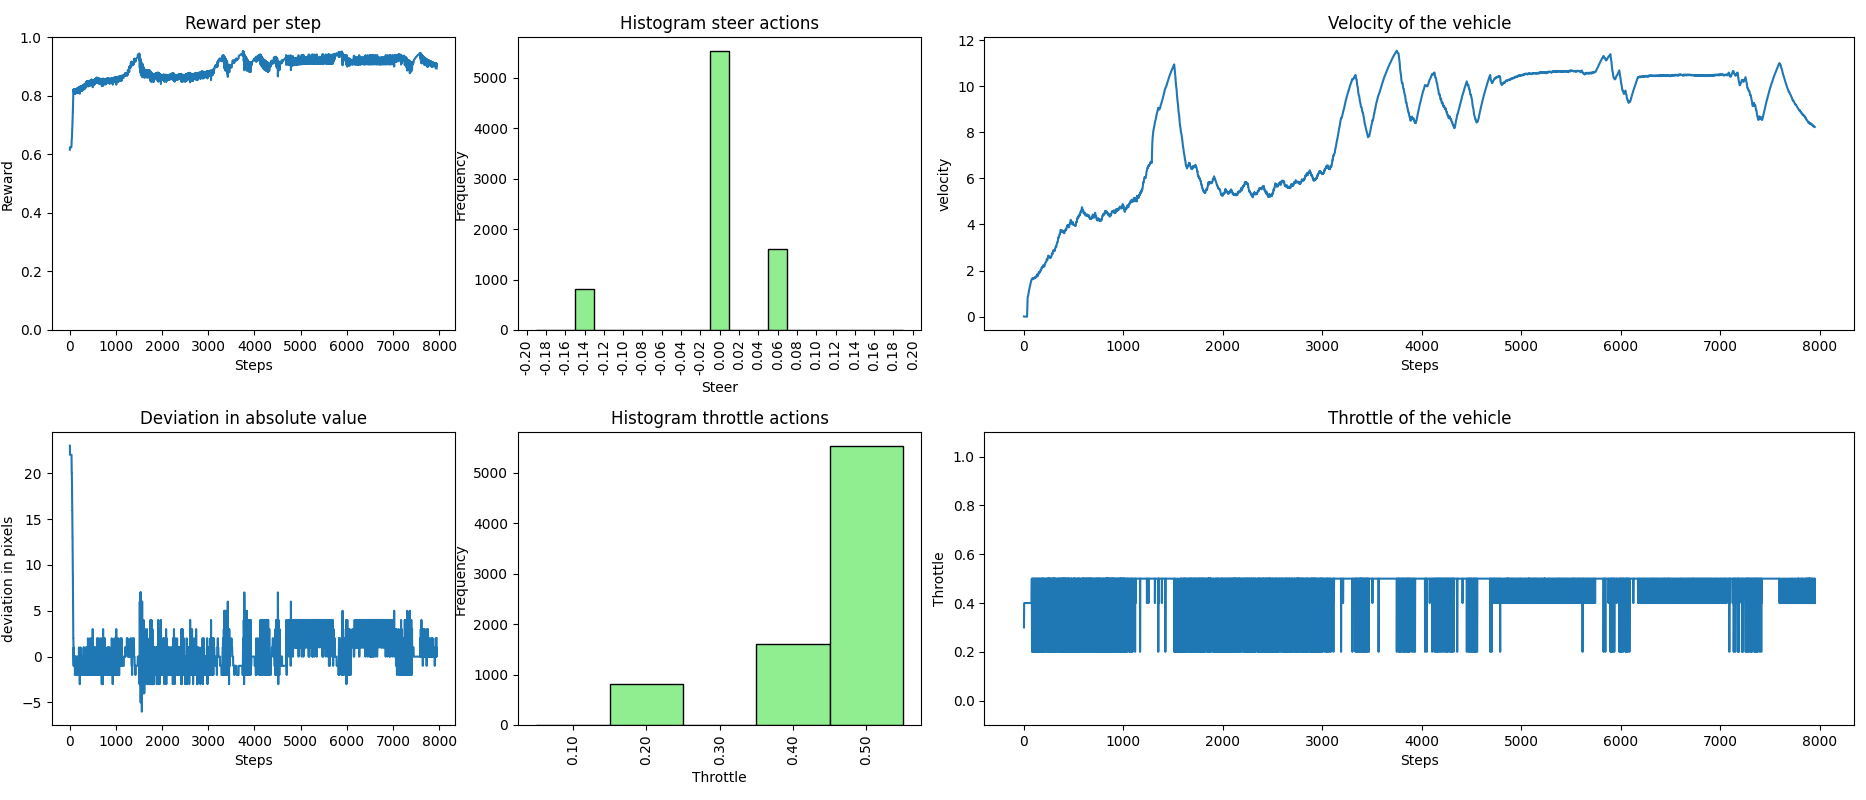
\includegraphics[width=14cm]{figs/Diseño/inference_dqn.png}
  \caption{Gráficas de inferencia sigue-carril basado en \ac{DQN}.}
  \label{fig:inference_dqn}
\end{figure}

\subsection{Seguimiento de carril con PPO}

El objetivo sigue siendo conseguir un seguimiento de carril fluido y la mayor velocidad posible, pero esta vez usamos el algoritmo \ac{PPO} que permite un espacio de acciones continuo. Se emplea la misma lógica para la finalización de un episodio, sensores, \textit{fixed\_delta\_seconds} de 50ms y circuito de entrenamiento \ref{fig:mapa} que en el entorno anterior.

- obs a fig en 4.2

\subsection{Control adaptativo con PPO}

\subsection{Maniobra de adelantamiento con PPO}

otro mapa